\documentclass[aspectratio=169]{beamer}
% Shared preamble for ml/ slide decks.
% Each lecture .tex starts with:
%   \documentclass[aspectratio=169]{beamer}
%   \input{../preamble}
% Compile from inside the chapter folder so \input{../preamble} resolves.

\usetheme{default}
\usecolortheme{dove}

\setbeamertemplate{navigation symbols}{}
\setbeamertemplate{footline}{%
  \hfill{\large\insertframenumber\,/\,\inserttotalframenumber}\hspace{0.8em}\vspace{0.5em}%
}

% Project palette (existing, kept for backwards compatibility with deferred/*)
\definecolor{popblue}{RGB}{52, 101, 164}
\definecolor{sampred}{RGB}{204, 0, 0}
\definecolor{paramgreen}{RGB}{0, 140, 70}
\definecolor{warnred}{RGB}{180, 40, 40}
\definecolor{orange1}{RGB}{220, 120, 0}
\definecolor{violet1}{RGB}{120, 50, 160}
\definecolor{lightbg}{RGB}{245, 245, 250}

% Armenian flag palette (use these for any 3-color highlight; per CLAUDE.md).
% "Nice versions": slightly de-saturated from the official spec for slide use,
% so they don't burn out under projector colors. Originals kept as *_pure.
\definecolor{armred}{RGB}{200, 30, 40}      % nice red (official #D90012 muted)
\definecolor{armblue}{RGB}{30, 70, 160}     % nice blue (official #0033A0 muted)
\definecolor{armorange}{RGB}{230, 160, 30}  % nice orange (official #F2A800 muted)
\definecolor{armred_pure}{HTML}{D90012}     % official Armenian flag red
\definecolor{armblue_pure}{HTML}{0033A0}    % official Armenian flag blue
\definecolor{armorange_pure}{HTML}{F2A800}  % official Armenian flag orange

\setbeamercolor{frametitle}{fg=popblue}
\setbeamercolor{title}{fg=popblue}

\usepackage{pgfplots}
\usepackage{tikz}
\usetikzlibrary{shapes, arrows.meta, positioning, calc, decorations.pathreplacing, patterns, matrix}
\pgfplotsset{compat=1.18}
\usepackage{amsmath, amssymb, amsfonts}
\usepackage{bm}
\usepackage{dsfont}
\usepackage{array}
\usepackage{pifont}
\usepackage{colortbl}
\usepackage{fontenc}

% Callout boxes. Purely additive - existing decks are unaffected.
% Usage: \begin{tcolorbox}[colback=armblue!8, colframe=armblue, boxrule=0.6pt, arc=2pt,
%                          title=\textbf{Key idea}] ... \end{tcolorbox}
% Palette convention (ml/SLIDE_STYLE.md): armblue=key idea, armred=trap/warning,
% paramgreen=takeaway or "Next", armorange=watch-out.
\usepackage[most]{tcolorbox}

% Cleaner table rules (\toprule, \midrule, \bottomrule). Also purely additive.
\usepackage{booktabs}

% \cancel{...} for struck-through terms in derivations (added 2026-08-11 for the
% importance-sampling frame in ch11_rl, where the dynamics cancel). Purely additive.
\usepackage{cancel}

% Minimal ML notation macros (subset of slds-lmu latex-math/basic-ml.tex).
% Kept here so we don't have to inline-expand every \thetav, \xv, etc.
% when porting upstream slides.
\newcommand{\R}{\mathds{R}}
\newcommand{\N}{\mathds{N}}
\newcommand{\E}{\mathds{E}}
\newcommand{\Xspace}{\mathcal{X}}
\newcommand{\Yspace}{\mathcal{Y}}
\newcommand{\Hspace}{\mathcal{H}}
\newcommand{\D}{\mathcal{D}}
\newcommand{\Dtrain}{\mathcal{D}_{\text{train}}}
\newcommand{\Dtest}{\mathcal{D}_{\text{test}}}
\newcommand{\xv}{\mathbf{x}}
\newcommand{\yv}{\mathbf{y}}
\newcommand{\Xmat}{\mathbf{X}}
\newcommand{\id}{\mathbf{I}}
\newcommand{\thetav}{\bm{\theta}}
\newcommand{\thetah}{\hat{\bm{\theta}}}
\newcommand{\lamv}{\bm{\lambda}}
\newcommand{\fx}{f(\xv)}
\newcommand{\fxt}{f(\xv \,|\, \bm{\theta})}
\newcommand{\fxi}{f\!\left(\xv^{(i)}\right)}
\newcommand{\fh}{\hat{f}}
\newcommand{\fxh}{\hat{f}(\xv)}
\newcommand{\yh}{\hat{y}}
\newcommand{\yih}{\hat{y}^{(i)}}
% \xi clashes with the Greek letter \xi; write \xv^{(i)} inline instead.
\newcommand{\yi}[1][i]{y^{(#1)}}
\newcommand{\xyi}[1][i]{\left(\xv^{(#1)},\, y^{(#1)}\right)}
\newcommand{\thx}{\bm{\theta}^\top \xv}
\newcommand{\sumin}{\sum_{i=1}^{n}}
\newcommand{\sumjp}{\sum_{j=1}^{p}}
\newcommand{\Lxy}{L\!\left(y, \fx\right)}
\newcommand{\Lxyi}{L\!\left(\yi, \fxi\right)}
\newcommand{\risk}{\mathcal{R}}
\newcommand{\riske}{\mathcal{R}_{\text{emp}}}
\newcommand{\risket}{\mathcal{R}_{\text{emp}}(\bm{\theta})}
\newcommand{\riskt}{\mathcal{R}(\bm{\theta})}
\newcommand{\riskr}{\mathcal{R}_{\text{reg}}}
\newcommand{\argmin}{\mathop{\mathrm{arg\,min}}}
\newcommand{\argmax}{\mathop{\mathrm{arg\,max}}}
\newcommand{\eps}{\varepsilon}


\usepackage{listings}
\lstset{
  basicstyle=\ttfamily\scriptsize,
  keywordstyle=\color{armblue}\bfseries,
  commentstyle=\color{paramgreen}\itshape,
  stringstyle=\color{armred},
  showstringspaces=false,
  language=Python,
  frame=single, framerule=0pt,
  backgroundcolor=\color{lightbg},
  numbers=none, breaklines=true, xleftmargin=4pt, xrightmargin=4pt,
}

\graphicspath{{fig/}{../00_shared/fig/}{../00_shared/fig/borrowed/}{../00_shared/fig/borrowed/3b1b/}{../00_shared/fig/borrowed/paper/}}

\newcommand{\bbb}{{\scriptsize\color{gray} 3Blue1Brown}}
\newcommand{\paper}[1]{{\scriptsize\color{gray} #1}}
\newcommand{\src}[1]{{\scriptsize\color{gray} #1}}
\newcommand{\link}[2]{\href{#1}{\textcolor{popblue}{#2}}}   % no underline: long titles must break

\newcommand{\bbbcap}[2]{%
  {\usebackgroundtemplate{\includegraphics[width=\paperwidth,height=\paperheight]{#1}}%
  \begin{frame}[plain]
    \begin{tikzpicture}[remember picture, overlay]
      \node[anchor=south west, font=\tiny, text=white!60]
        at ([shift={(0.26cm,0.16cm)}]current page.south west) {3Blue1Brown};
      \node[anchor=south, font=\small\itshape, text=white, fill=black!60,
            inner sep=5pt, rounded corners, text width=0.86\paperwidth, align=center]
        at ([shift={(0,0.85cm)}]current page.south) {#2};
    \end{tikzpicture}
  \end{frame}}%
}

\newcommand{\keybox}[1]{\fcolorbox{armblue}{armblue!8}{\parbox{0.97\linewidth}{\small #1}}}
\newcommand{\trapbox}[1]{\fcolorbox{armred}{armred!8}{\parbox{0.97\linewidth}{\small #1}}}
\newcommand{\takebox}[1]{\fcolorbox{paramgreen}{paramgreen!8}{\parbox{0.97\linewidth}{\small #1}}}
\newcommand{\watchbox}[1]{\fcolorbox{armorange}{armorange!12}{\parbox{0.97\linewidth}{\small #1}}}

\newcommand{\sectiontransition}[2]{%
  \begin{frame}[plain]
    \vfill
    \begin{center}
      {\Huge\bfseries\color{popblue} #1}\\[1.1em]
      {\large #2}
    \end{center}
    \vfill
  \end{frame}}

\title{Transformers in the World}
\subtitle{The family, the LM head, and what it costs}
\author{}
\date{}

\begin{document}

\begin{frame}[plain]
  \titlepage
\end{frame}

% ============================================================ LINKS (2026-10-27, as in LLM-1 to LLM-4)
\begin{frame}{Before we start: videos and a demo}
  \begin{columns}[T]
    \column{0.49\textwidth}
    \keybox{\raggedright\textbf{Recommended viewing}\\[4pt]
    Hugging Face's course, three short videos (16 min in all):
    \link{https://www.youtube.com/watch?v=MUqNwgPjJvQ}{Transformer models: Encoders},
    \link{https://www.youtube.com/watch?v=d_ixlCubqQw}{Transformer models: Decoders},
    \link{https://www.youtube.com/watch?v=0_4KEb08xrE}{Transformer models: Encoder-Decoders}.
    Today's first section.\\[6pt]
    3Blue1Brown, \link{https://youtu.be/wjZofJX0v4M?t=1222}{Transformers, the tech
    behind LLMs \textbar{} Deep Learning Chapter 5}, from 20:22: the unembedding, then softmax with
    temperature (22:22). Today's second section, and LLM-6's opening.}
    \column{0.49\textwidth}
    \takebox{\raggedright\textbf{Live demo:}
    \link{https://bbycroft.net/llm}{bbycroft.net/llm}\\[4pt]
    Brendan Bycroft's LLM Visualization: every matrix of a transformer in 3D. A guided walk
    through a tiny model, then GPT-2 small, GPT-2 XL and GPT-3, drawn to scale.}
    \vskip 4pt
    {\small\textbf{Try:}}
    \begin{itemize}\small
      \item the walk-through, up to ``Output''
      \item GPT-2 small next to GPT-3: the same block, bigger
      \item find the LM head at the very end
    \end{itemize}
  \end{columns}
\end{frame}

% ============================================================ WHERE WE ARE (py_src/llm_roadmap.py)
\begin{frame}{Where we are: one forward pass}
  \begin{center}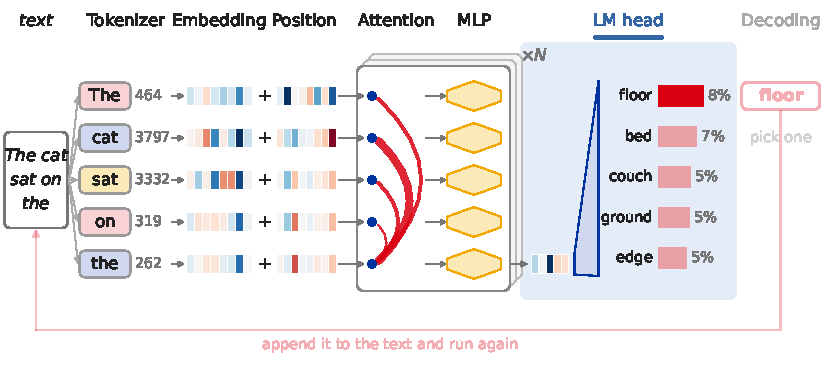
\includegraphics[width=\linewidth]{roadmap_transformers_pass.pdf}\end{center}
  \vskip -2pt
  {\small Today: the \textbf{LM head} (last vector to a distribution) and three ways to wire the
  block.}
\end{frame}

\begin{frame}{Where we are: the life of a model}
  \begin{center}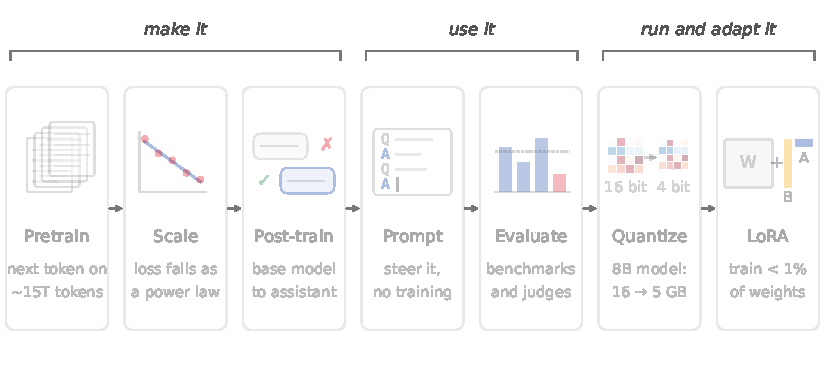
\includegraphics[width=\linewidth]{roadmap_transformers_life.pdf}\end{center}
  \vskip -2pt
  {\small Later: where these weights come from, and what you do with them once you have them.}
\end{frame}

% ============================================================ COLD OPEN (py_src/head_figs.py)
\begin{frame}{Which of these can write text?}
  \vskip 2pt
  Three attention masks for the same block. A row is the token being computed; the shaded cells
  are the tokens it may look at.

  \vskip 4pt
  \begin{center}
    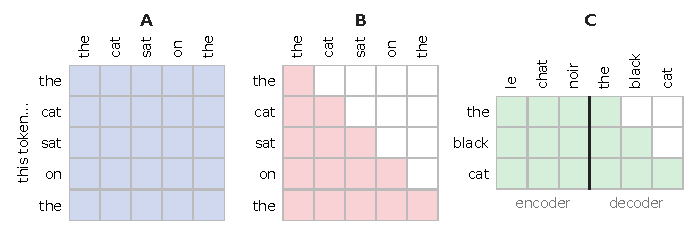
\includegraphics[width=0.84\linewidth]{head_masks.pdf}
  \end{center}

  \vskip -2pt
  \keybox{\textbf{Predict first:} which of A, B, C could \emph{write} a sentence, left to right,
  one token at a time? More than one answer is allowed.}
\end{frame}

\begin{frame}{B and C can. A cannot.}
  \vskip 2pt
  \begin{center}
    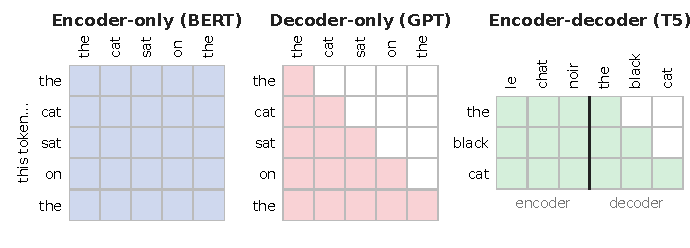
\includegraphics[width=0.84\linewidth]{head_masks_named.pdf}
  \end{center}

  \vskip -4pt
  {\small \textbf{A} lets the first ``the'' look at ``sat''. When you write, word 3 does not exist
  yet while you choose word 2, so a model trained to peek cannot be run forwards.
  \textbf{B} is LLM-4's causal mask. \textbf{C} writes English with a causal mask too, and also
  reads the whole French sentence (drawn as one grid; in the model it is two attention
  layers, one over each sequence).}

  \vskip 4pt
  \keybox{The block is the same in all three. The difference is one decision:
  \textbf{who is allowed to look at whom?}}
\end{frame}

\begin{frame}{Outline}
  \tableofcontents
\end{frame}

% ============================================================ SECTION 1
\section{The family}
\sectiontransition{The family}{One block, three ways of wiring it.}

\begin{frame}{The original: an encoder and a decoder}
  \vskip 4pt
  \begin{columns}[T]
    \column{0.40\textwidth}
      \vskip -2pt
      % Figure 1 sits at roughly x 206-432pt, y 381-728pt on the 612x792pt page.
      % trim is left/bottom/right/top, so cut everything outside that box.
      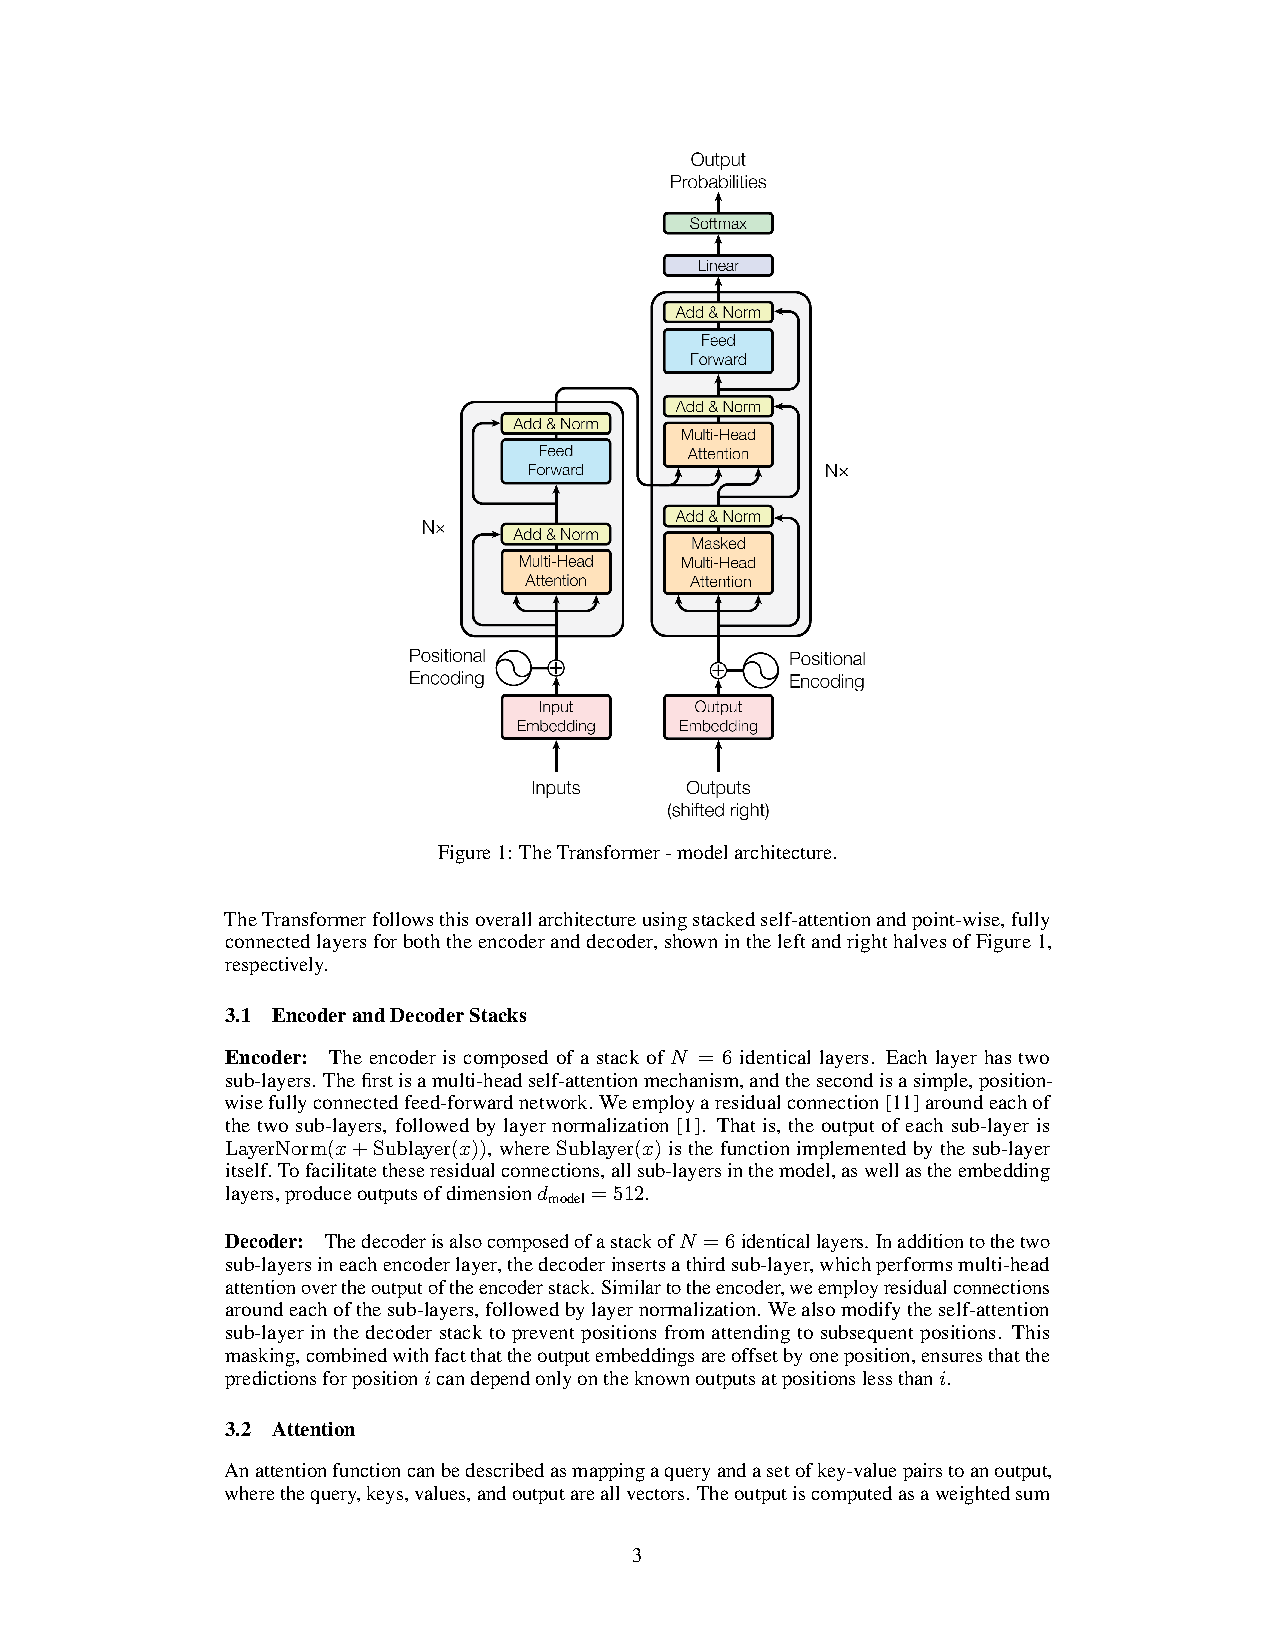
\includegraphics[height=0.62\textheight, keepaspectratio,
                       trim=195 402 170 55, clip]{vaswani_fig1_page.pdf}\\
      \paper{Vaswani et al. (2017), Figure 1}
    \column{0.57\textwidth}
      \vskip 8pt
      {\small The 2017 paper was about \textbf{translation}, so it has two stacks:

      \vskip 6pt
      \textbf{Encoder} -- reads the source sentence. Every token may see every other token.

      \vskip 6pt
      \textbf{Decoder} -- writes the target sentence, one token at a time, so it is
      \textbf{causally masked} (LLM-4).

      \vskip 8pt
      They are joined by \textbf{cross-attention}: the decoder supplies the queries, and the
      \emph{encoder's} output supplies the keys and values.}
  \end{columns}

  \vskip 0pt
  \keybox{Self-attention asks ``what in \emph{this} sentence matters to me?'' Cross-attention
  asks ``what in \emph{that other} sequence matters to me?'' Identical mechanism; the keys and
  values just come from somewhere else.}
\end{frame}

\begin{frame}{Cross-attention, with actual numbers}
  \vskip 2pt
  The decoder is writing an English sentence and has produced ``the''. The encoder has already
  read the French source. Where should ``the'' look?

  \vskip 4pt
  \begin{center}
    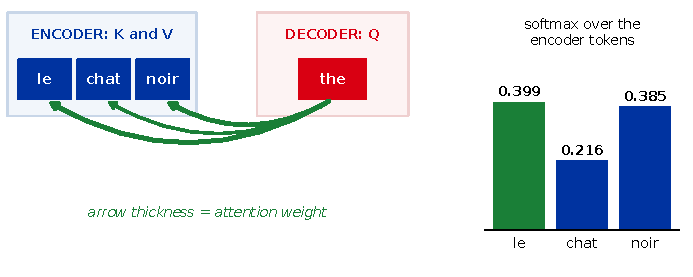
\includegraphics[width=0.80\linewidth]{head_cross_attention.pdf}
  \end{center}

  \vskip -2pt
  {\footnotesize One head, $d_k = 4$, toy random weights. Each score is $q \cdot k / \sqrt{4}$:
  for ``le'', $0.6788 / 2 = 0.3394 \approx +0.339$; the others are $-0.273$ and $+0.304$. Softmax
  gives \textbf{0.399}, \textbf{0.216}, \textbf{0.385} (sum 1), and the output is
  $0.399\,v_{\text{le}} + 0.216\,v_{\text{chat}} + 0.385\,v_{\text{noir}}$, exactly as in LLM-3.}
\end{frame}

\begin{frame}{What actually changed}
  \vskip 2pt
  Compare with the self-attention you computed in LLM-3. The formula is character-for-character
  the same:
  \vskip 4pt
  \begin{center}
    $\text{Attention}(Q, K, V) = \text{softmax}\!\left(\dfrac{QK^\top}{\sqrt{d_k}}\right) V$
  \end{center}

  \vskip 8pt
  \begin{center}
  \small
  \begin{tabular}{lll}
    \toprule
    & \textbf{Self-attention} & \textbf{Cross-attention} \\
    \midrule
    $Q$ comes from & this sequence & \textbf{the decoder} \\
    $K, V$ come from & this sequence & \textbf{the encoder} \\
    \bottomrule
  \end{tabular}
  \end{center}

  \vskip 6pt
  {\small Where it sits: every decoder block has \textbf{three} sublayers - masked
  self-attention, then cross-attention (its own $W_Q, W_K, W_V$; the keys and values come from
  the encoder's \emph{final} output, the same for every decoder block), then the MLP.}

  \vskip 6pt
  \keybox{That is the entire difference: \textbf{two of the three inputs come from somewhere
  else}. No new mechanism, no new maths -- which is why the original paper could reuse the same
  block for both.}
\end{frame}

\begin{frame}{Three architectures}
  \vskip 4pt
  \begin{center}
    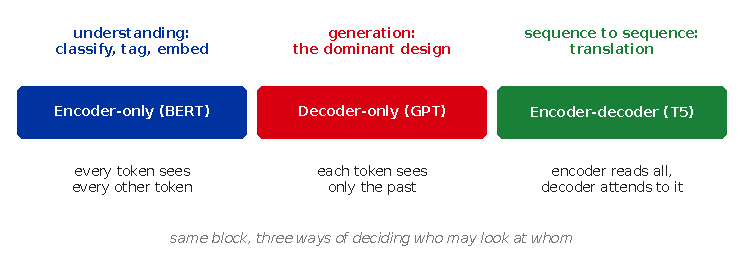
\includegraphics[width=0.90\linewidth]{head_three_arch.pdf}
  \end{center}
  \vskip -2pt
  \takebox{Nobody changed the block. \textbf{Encoder-only} sees in both directions and is good
  at understanding: BERT is trained to fill in hidden words, with both sides visible.
  \textbf{Decoder-only} sees only backwards, which makes it able to generate.
  \textbf{Encoder-decoder} keeps both and joins them with cross-attention.}
\end{frame}

\begin{frame}{The family, by name}
  \begin{itemize}
    \item \textbf{Encoder-only}: BERT (Google, 2018). Not retired: ModernBERT (December 2024)
      was trained on 2 trillion tokens, reads 8,192 tokens at once, and is built for
      classification and retrieval - the embeddings that retrieval-augmented generation (RAG)
      needs.
    \item \textbf{Encoder-decoder}: T5 (Raffel et al., 2020) turns every task into text in, text
      out, with a prefix that names the task: ``translate English to German: That is good.''
      $\to$ ``Das ist gut.''; ``mnli premise: I hate pigeons. hypothesis: My feelings towards
      pigeons are filled with animosity.'' $\to$ ``entailment''. Pretrained by blanking out spans
      of text and writing them back.
    \item \textbf{Decoder-only}: GPT-2, and every chat model you have used.
  \end{itemize}
  \vskip 6pt
  \watchbox{A running joke of 2018-2020: ELMo (2018), BERT (2018), ERNIE (2019), Grover (2019),
  KERMIT (2019), Big Bird (2020). For a while, language models were named after Sesame Street.}
\end{frame}

\begin{frame}{Why decoder-only won the last five years}
  \vskip 8pt
  \begin{itemize}
    \item \textbf{One objective, every token.} BERT's fill-in-the-blank needs no labels either,
      but it learns only from the 15\% of tokens it hides, and it cannot write. Next-token
      prediction learns from every token (LLM-4's mask), and the model it trains writes.
    \item \textbf{It subsumes the others.} ``Translate this: \ldots'' is just a prompt. Tasks
      that needed a separate architecture became a formatting question.
    \item \textbf{It is the simplest thing to scale.} One stack, one loss, no encoder to keep
      in sync.
  \end{itemize}

  \vskip 10pt
  \watchbox{This is a statement about the last few years, not a theorem. Encoder-only models
  are still the right tool when you want an \emph{embedding} rather than a continuation -- which
  is exactly what the retrieval chapter (RAG, after LLM-11) will use them for.}
\end{frame}

\begin{frame}{Mask A writes after all: diffusion language models}
  \begin{itemize}
    \item Mask A failed because word 3 does not exist yet while word 2 is chosen. A diffusion
      language model makes every position exist from the start: the answer has a fixed length and
      begins as all blanks. That is BERT's fill-in-the-blank, run again and again.
    \item Each step predicts every blank at once, keeps the guesses the model is most sure of
      (highest probability), blanks the rest again, and repeats for a set number of steps.
    \item LLaDA (Nie et al., NeurIPS 2025): 8B parameters, ``does not use a causal mask'';
      ``competitive with'' LLaMA 3 8B. The selling point is speed, many tokens per step: Mercury
      (2025) and Google's open DiffusionGemma (2026), with quality a step behind.
  \end{itemize}
  \vskip 6pt
  \watchbox{The cold open's answer holds for writing one token at a time. Write everything at
  once and refine it, and mask A works - so far trading some quality for speed.}
  \vskip 2pt
  \src{Nie et al., arXiv 2502.09992; Inception Labs (Feb 2025: over 1,000 tokens/s on one GPU);
  Google (10 June 2026: up to 4$\times$ faster, quality below Gemma 4).}
\end{frame}

% ============================================================ SECTION 2 (py_src/head_figs.py --gpt2)
\section{The LM head}
\sectiontransition{The LM head}{From the last vector to a probability for every token.}

\bbbcap{snape_prediction.png}{Next-token prediction, in practice: the model outputs a
distribution over the whole vocabulary, and one continuation is far more likely than the rest.}

\begin{frame}{From a vector to a word}
  \vskip 4pt
  \begin{columns}[T]
    \column{0.46\textwidth}
      \vskip -4pt
      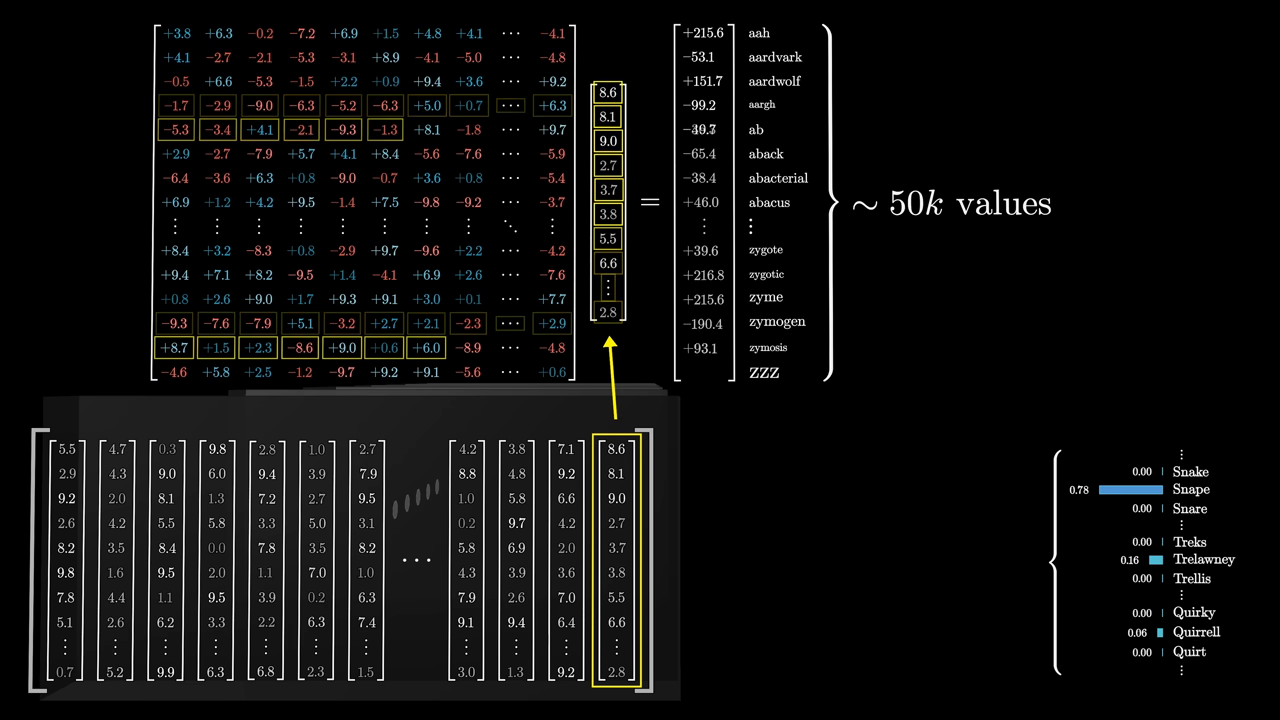
\includegraphics[width=\linewidth]{unembedding_matrix.png}\\ \bbb
    \column{0.50\textwidth}
      \vskip -2pt
      {\small Every position leaves the last block with a vector. In training, every one of
      them predicts its own next token at once (LLM-4's mask keeps that honest). When
      generating, the earlier next tokens are already written, so only the \textbf{last}
      vector's prediction is new. After one final LayerNorm it is multiplied by an
      \textbf{unembedding matrix} -- one row per vocabulary entry, so roughly 50,000 numbers
      come out.

      \vskip 6pt
      Those are \textbf{logits}. A softmax turns them into a probability distribution, and you
      sample from it. That is the entire output stage.}
  \end{columns}

  \vskip 4pt
  \keybox{The model produces a \emph{distribution} over every word, not a word. Choosing is a
  separate decision: temperature and the other decoding strategies (LLM-6).}
\end{frame}

\begin{frame}{GPT-2's head, on the map's prompt}
  \begin{center}
    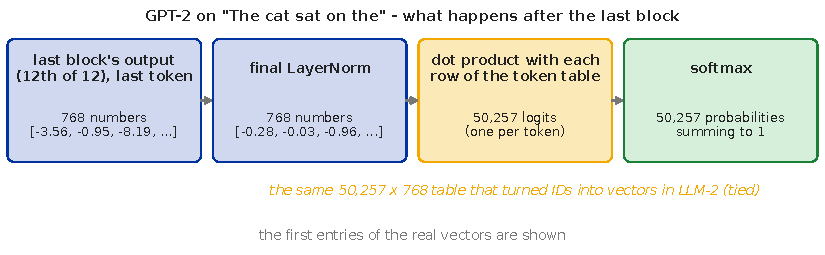
\includegraphics[width=0.93\linewidth]{head_pipeline.pdf}
  \end{center}

  \vskip -2pt
  {\small The ``unembedding matrix'' in GPT-2 is not a new matrix. It is the token table from
  LLM-2, used a second time: \textbf{tied}. Row $j$ turned token $j$ into a vector on the way in;
  on the way out, its dot product with the last vector scores token $j$. Both jobs want tokens
  used alike to get vectors alike (LLM-2).}

  \vskip 4pt
  \takebox{The table is $50{,}257 \times 768 = 38.6$M numbers, \textbf{31\%} of GPT-2's 124.4M
  parameters. Tying it means the head costs no parameters of its own.}
\end{frame}

\begin{frame}{What comes out}
  \vskip 2pt
  \begin{columns}[c]
    \column{0.62\textwidth}
      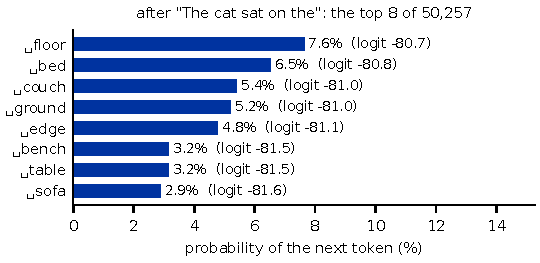
\includegraphics[width=\linewidth]{head_top_tokens.pdf}
    \column{0.36\textwidth}
      {\small Real output of the cached GPT-2 small. ($\textvisiblespace$ is the leading space,
      part of the token: LLM-1.)

      \vskip 6pt
      The top five hold \textbf{30\%} of the probability. Only \textbf{14} of the 50,257 tokens
      get more than 1\%; the remaining mass is spread thinly over everything else.

      \vskip 6pt
      And look at the logits: \textbf{all of them are near $-80$}.}
  \end{columns}

  \vskip 6pt
  \keybox{\textbf{Predict:} if every logit is around $-80$, how can ``floor'' end up with 7.6\%?}
\end{frame}

\begin{frame}{One logit, by hand}
  \vskip 4pt
  {\small\textbf{A logit is one dot product}, 768 terms long: the last vector against one row of
  the token table. For the token ``floor'':}
  \par\vskip 6pt
  {\footnotesize
  \hspace*{1em}$z(\text{floor}) = (-0.284)(-0.122) + (-0.033)(0.161) + (-0.962)(-0.025)
  + (0.225)(-0.024) + \ldots$
  \par\vskip 4pt
  \hspace*{1em}The first four terms give $0.048$; all 768 give $z(\text{floor}) = -80.65$.
  Likewise $z(\text{bed}) = -80.81$.}

  \vskip 12pt
  \keybox{Every row of the table gets its own dot product: 50,257 of them, which is one matrix
  multiplication. A row that points more the same way as the last vector gets a \textbf{higher}
  score than the others - here they all sit around $-80$, and only the differences count.}

  \vskip 8pt
  {\small Every logit is near $-80$. Back to the question: how does ``floor'' end up with 7.6\%?}
\end{frame}

\begin{frame}{Answer: only differences matter}
  {\small\textbf{Two tokens: compare them directly.}}
  \par\vskip 3pt
  {\footnotesize
  \hspace*{1em}$\dfrac{p(\text{floor})}{p(\text{bed})}
  = \dfrac{\exp z(\text{floor})}{\exp z(\text{bed})}
  = \exp\big(z(\text{floor}) - z(\text{bed})\big) = \exp(0.157) = 1.17$
  \par\vskip 2pt
  \hspace*{1em}Check against the bars: $7.64\% \,/\, 6.53\% = 1.17$.}

  \vskip 8pt
  {\small\textbf{One token: compare it with all of them.}}
  \par\vskip 3pt
  {\footnotesize
  \hspace*{1em}$p(\text{floor}) = \dfrac{\exp z(\text{floor})}{\sum_{j} \exp z_j}
  = \exp\big(z(\text{floor}) - \log\textstyle\sum_j \exp z_j\big)$
  \quad ($j$ runs over all 50,257 tokens)
  \par\vskip 3pt
  \hspace*{1em}$\phantom{p(\text{floor})} = \exp\big(-80.654 - (-78.082)\big) = \exp(-2.572)
  = \mathbf{7.64\%}$
  \par\vskip 3pt
  \hspace*{1em}$\log\sum_j \exp z_j = -78.08$ sits \emph{above} the largest logit ($-80.65$):
  50,257 positive terms add up to more than the largest one alone.}

  \vskip 8pt
  \keybox{\raggedright Add the same number $c$ to every logit and nothing changes:
  $e^{z_i + c} / \sum_j e^{z_j + c} = e^{z_i} / \sum_j e^{z_j}$, because the factor $e^{c}$
  cancels. The softmax only sees \textbf{differences}. That is why $-80$ is harmless,
  and it is the knob LLM-6 turns: temperature stretches or shrinks those differences.}
\end{frame}

\begin{frame}{By hand: three logits near $-80$}
  \small
  Three tokens with logits $(-80,\ -81,\ -82)$. Subtract the largest from all three: $(0,\ -1,\ -2)$.
  \[
    \text{softmax} = \frac{(e^{0},\ e^{-1},\ e^{-2})}{e^{0} + e^{-1} + e^{-2}}
    = \frac{(1,\ 0.37,\ 0.14)}{1.50} = (\mathbf{0.67},\ 0.24,\ 0.09)
  \]
  The same as for $(-80, -81, -82)$, because the shift cancels. That is also how code computes a
  softmax safely: subtract the largest logit first (LLM-3's ten lines did), so no $e^{z}$
  overflows or underflows.
  \vskip 6pt
  \textbf{Back to GPT-2.} The denominator's log, $\log\sum_j e^{z_j} = -78.08$, has a name:
  \textbf{log-sum-exp}. It sits $2.57$ above floor's $-80.65$, so all 50,257 tokens together carry
  $e^{2.57} = 13.1$ times floor's weight, and floor gets $1 / 13.1 = 7.6\%$.
  \vskip 6pt
  \keybox{Floor is the single favourite, but the other 50,256 tokens together outweigh it about
  12 to 1. LLM-6 starts from exactly that tail.}
\end{frame}

% ============================================================ SECTION 3
\section{Why it won, and what it costs}
\sectiontransition{Why it won, and what it costs}{Every architecture buys something with
something.}

\begin{frame}{Why transformers won}
  \vskip 2pt
  \begin{enumerate}
    \item[\textbf{1.}] \textbf{It parallelises.} An RNN had to walk the sequence in order.
      Attention is a few big matrix multiplications over the whole sequence at once (LLM-3),
      which is exactly the workload a GPU wants. That is training; generating is still one
      token at a time (LLM-6).
    \item[\textbf{2.}] \textbf{Because it parallelises, it scales.} You can afford more data and
      more parameters.
    \item[\textbf{3.}] \textbf{Because it scales, it kept getting better.} The clearest example
      is \textbf{in-context learning}: give a model a few examples in the prompt and it follows
      the pattern, \emph{with no weight updates at all} (``cat $\to$ chat, dog $\to$ chien,
      bird $\to$'' gets ``oiseau''). Small models do it badly, large ones
      well; whether that improvement is sudden or gradual is debated (LLM-8).
  \end{enumerate}

  \vskip 6pt
  \keybox{Notice the shape of that argument: the win is not that attention is a cleverer model
  of language. It is that attention is a \textbf{better fit for the hardware}, and everything
  else followed from being able to train bigger. Architecture that suits the machine beats
  architecture that suits your intuition.}
\end{frame}

\begin{frame}{The bill: attention is quadratic}
  \vskip 4pt
  Every token attends to every token, so the score matrix is $n \times n$. Double the context
  and you quadruple that cost.

  \vskip 4pt
  \begin{center}
    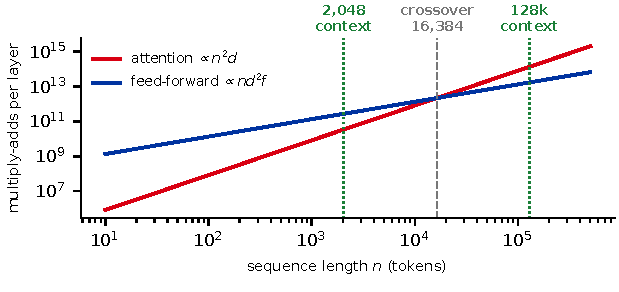
\includegraphics[width=0.75\linewidth]{head_quadratic.pdf}
  \end{center}

  \vskip -2pt
  {\small $d_{\text{model}} = 4096$, $f = 4$. The grid costs memory too: at 128,000 tokens one
  head's $n \times n$ scores are 16.4 billion numbers, so FlashAttention never stores it whole
  (LLM-14).}
\end{frame}

\begin{frame}{Read that graph carefully}
  \vskip 4pt
  The usual story is ``attention is the bottleneck''. The arithmetic says: \textbf{not until
  the sequence gets long}.

  \vskip 2pt
  You can work out where it flips in two lines. Attention's $n \times n$ part costs about
  $n^2 d$ (only the $n \times n$ part; the Q, K, V and output projections grow like the
  feed-forward and would only push the crossover further out); the feed-forward costs about
  $n d^2 f$, where $f$ is the widening factor
  (usually 4). Set them equal:
  \vskip 2pt
  \begin{center}
    $n^2 d = n d^2 f \quad\Longrightarrow\quad \boxed{n = d \cdot f}$
  \end{center}

  \vskip 4pt
  So for $d_{\text{model}} = 4096$ and $f = 4$, the crossover is at
  $4096 \times 4 = \mathbf{16{,}384}$ tokens. Halve the model and you halve the crossover. For
  GPT-2 small, $768 \times 4 = 3{,}072$: three times its whole 1{,}024-token window.

  \vskip 4pt
  \watchbox{So for a 2,048-token context, optimising attention is optimising the smaller half.
  ``Quadratic'' describes how the cost \emph{grows}, not where the cost \emph{is} at every
  size. FlashAttention and sparse variants attack the $n^2$ term; 2025 hybrids keep full
  attention in a quarter of their layers or fewer (LLM-14).}
\end{frame}

\begin{frame}{The honest limit: almost no inductive bias}
  An \textbf{inductive bias}: what a model assumes before it sees any data. Every model here had one:

  \vskip 2pt
  \begin{center}
  \footnotesize
  \begin{tabular}{lll}
    \toprule
    \textbf{Model} & \textbf{Built-in assumption} & \textbf{Consequence} \\
    \midrule
    Decision tree & axis-aligned splits matter & works on tiny tabular data \\
    CNN & nearby pixels are related & learns vision from thousands of images \\
    RNN & order matters, recent matters more & handles sequences by construction \\
    \textbf{Transformer} & \textbf{almost nothing} & \textbf{needs enormous data} \\
    \bottomrule
  \end{tabular}
  \end{center}

  \vskip 2pt
  A Transformer does not know that neighbouring words are related, or even that words have an
  order -- we had to \emph{bolt position on} in LLM-2. Its only built-in assumptions are the
  ones we add by hand: positions, and the causal mask.

  \vskip 3pt
  \trapbox{That weakness is the same fact as its strength. Assuming nothing means it can learn
  any structure, and \textbf{must} learn all of it from data. This is why a ViT loses to a CNN
  on a small image dataset and wins on a huge one (Dosovitskiy et al., 2021: behind ResNets on
  ImageNet alone, ahead after 14-300M images), and why transformers arrived only once
  the data and the compute did.}
\end{frame}

\begin{frame}{Same block, everywhere}
  \vskip 2pt
  \begin{center}
  \small
  \begin{tabular}{lll}
    \toprule
    \textbf{Domain} & \textbf{What became a token} & \textbf{Chapter} \\
    \midrule
    Text & subword pieces & this chapter \\
    Images (ViT) & 16$\times$16 patches & vision-language models \\
    Audio & spectrogram frames or codec codes & audio \\
    Proteins & amino acids & protein language models, AlphaFold \\
    Actions & robot commands & vision-language-action \\
    \bottomrule
  \end{tabular}
  \end{center}

  \vskip 4pt
  \takebox{Nobody redesigned the block for any of these. They redesigned what counts as a
  \textbf{token}. That is the practical legacy of the architecture: if you can serialise your
  problem into a sequence of vectors, you can throw a Transformer at it.}
  \vskip 4pt
  {\small AlphaFold 2 is built on attention. Half of the 2024 Nobel Prize in Chemistry went to its
  makers, Demis Hassabis and John Jumper, ``for protein structure prediction''.}
\end{frame}

% ============================================================ RECAP
\begin{frame}{Recap}
  \vskip 4pt
  \small
  \begin{itemize}
    \item \textbf{One block, three wirings.} Encoder-only (BERT) understands, decoder-only (GPT)
      generates, encoder-decoder (T5) translates. The difference is who may look at whom - the
      mask, plus cross-attention in the decoder - not the attention itself.
    \item \textbf{Cross-attention} is ordinary attention with the keys and values taken from
      another sequence. Diffusion LMs write with no causal mask at all, many tokens per step.
    \item \textbf{The LM head} is one dot product per vocabulary entry with the token table
      (tied in GPT-2), then a softmax. The output is a distribution, not a word, and only the
      differences between logits matter.
    \item \textbf{It won because it fits the GPU}, not because it is a better theory of language.
    \item \textbf{It is quadratic in sequence length}, but at $d_{\text{model}}=4096$ that only
      dominates past 16,384 tokens.
    \item \textbf{It assumes almost nothing}, so it can learn anything and needs vast data to
      do it.
  \end{itemize}
\end{frame}

\begin{frame}{Next on the map}
  \begin{center}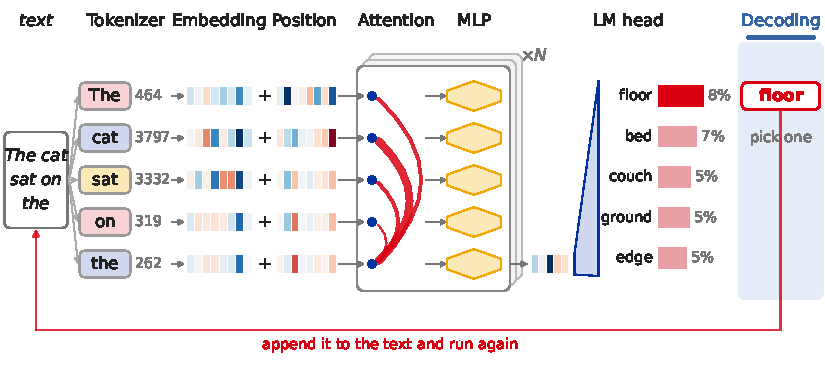
\includegraphics[width=\linewidth]{roadmap_decoding_pass.pdf}\end{center}
  \vskip -2pt
  {\small Next (LLM-6): \textbf{decoding} - how a distribution becomes the text you read.}
\end{frame}

\begin{frame}{Sources \& further reading}
  \footnotesize
  \begin{itemize}
    \item \textbf{Watch:} Hugging Face course (2021), ``Transformer models: Encoders / Decoders /
      Encoder-Decoders''; 3Blue1Brown (2024), Deep Learning Chapter 5. \textbf{Play:}
      \link{https://bbycroft.net/llm}{bbycroft.net/llm}.
    \item Vaswani et al. (2017), ``Attention Is All You Need'', NeurIPS (the encoder-decoder,
      cross-attention).
    \item Devlin et al. (2019), ``BERT'', NAACL; Raffel et al. (2020), ``Exploring the Limits of
      Transfer Learning with a Unified Text-to-Text Transformer'' (T5), JMLR; Warner et al. (2025),
      ``ModernBERT'', ACL.
    \item Radford et al. (2019), ``Language Models are Unsupervised Multitask Learners'' (GPT-2).
    \item Nie et al. (2025), ``Large Language Diffusion Models'' (LLaDA), NeurIPS.
    \item Dosovitskiy et al. (2021), ``An Image is Worth 16x16 Words'' (ViT), ICLR; Jumper et al.
      (2021), ``Highly accurate protein structure prediction with AlphaFold'', \emph{Nature}.
    \item Qwen team (2025), Qwen3-Next model card; Moonshot AI (2025), ``Kimi Linear''; NVIDIA
      (2025), ``Nemotron-H''.
  \end{itemize}
  \vskip 2pt
  \src{GPT-2's head: \texttt{py\_src/head\_figs.py} (cached GPT-2 small, raw results in
  \texttt{results/head\_gpt2.json}).}
\end{frame}

\end{document}

% ============================================================================
% Provenance
%
% PLAN: llms/ATTENTION_CHAPTER_PLAN.md, section "L26", approved 2026-07-19.
% Frame order follows that outline. The 2026 applications montage became a TABLE ("same block,
% everywhere") rather than a web-image montage - it makes the same point, needs no external
% images, and doubles as a map of where the rest of the course uses transformers.
%
% SOURCES:
%   - misc/dl4nlp/02_transformers.tex - the encoder/decoder/cross-attention treatment, the three
%     architectures, "how transformers learn", "why transformers won", and the complexity frame.
%   - 3Blue1Brown Ch5, frames in fig/borrowed/3b1b/: snape_prediction.png, unembedding_matrix.png.
%     Credit line only, per the instructor's 2026-07-21 decision.
%   - Vaswani et al. (2017), arXiv 1706.03762. Page 3 extracted with pypdf to
%     fig/borrowed/paper/vaswani_fig1_page.pdf and cropped to Figure 1 on the slide.
%
% FIGURES - py_src/l25_l26_figs.py:
%   REAL:
%     l26_quadratic - attention FLOPs (2 n^2 d) against feed-forward FLOPs (2 n d^2 f), computed.
%       The crossover is solved rather than eyeballed: n = d * f = 16,384 tokens for d=4096, f=4.
%       This produced the "read that graph carefully" frame, which is NOT in the approved plan:
%       the arithmetic contradicts the usual "attention is the bottleneck" summary at typical
%       context lengths, and that seemed worth a frame of its own.
%   ILLUSTRATIVE (labelled "schematic" on the figure):
%     l26_three_arch - encoder-only / decoder-only / encoder-decoder.
%
% DELIBERATE CHOICES:
%   - "Why decoder-only won" carries an explicit hedge that it is a statement about the last few
%     years, not a theorem, and points at the retrieval chapter's use of encoder-only models.
%   - The inductive-bias frame completes the ledger started in ch4 (trees), ch6 (CNN) and ch7
%     (RNN), as the plan intended. It is framed as strength and weakness being the same fact.
%
% NOT DONE:
%   - Decoding strategies (temperature, top-k, nucleus) are teased once and left to the later
%     part of the chapter, per the plan.
%   - No homework frame; the numpy attention exercise lives on attention.qmd.
%   REVISION 2026-10-04: two "Where we are" frames after the title (one forward pass; the life
%   of a model) and "Next on the map" before the closing frame
%   (fig/roadmap_transformers_pass/_life.pdf, roadmap_decoding_pass.pdf from
%   py_src/llm_roadmap.py). Tokenization now comes before L24, so the closing frame's
%   "Next in this chapter" lost it and starts with decoding (DECISIONS #67).
%   RENAMED 2026-10-05 (DECISIONS #71, the chapter renumbered in teaching order): L26_transformers_in_the_world.tex -> LLM5_transformers_in_the_world.tex.
%   Labels in the body were renumbered by script; this provenance block keeps the old names.
%   RESTRUCTURE 2026-10-06 (INTERVIEW_QUEUE.md, LLM-5, the recommended answers; instructor: "do all
%   queue items"): cold open is now predict-first - three unnamed masks, "which can write text?",
%   then the answer (B and C). "How it learns" is cut: its objective frame lives in LLM-4 (the mask)
%   and LLM-7 (pretraining), "autocomplete is not a chatbot" opens LLM-9. In its place, "The LM
%   head": the 3b1b still and the unembedding frame stay, plus GPT-2's real head on the map's
%   prompt (pipeline, top-8, the head by hand: one logit as a 768-term dot product, the ratio
%   e^0.157 = 1.17, p = e^-2.572 = 7.64%). The [plain] "That is the T in GPT" ending is gone.
%   FIGURES now from py_src/head_figs.py, drawn at slot size: head_masks(_named), head_pipeline,
%   head_top_tokens (REAL, cached GPT-2, results/head_gpt2.json; every printed number checked),
%   and head_cross_attention / head_three_arch / head_quadratic, ports of the l26_* figures
%   (same seed and numbers; the l26_* PDFs and l25_l26_figs.py stay for the record).
%   STUDENT REVIEW 2026-10-06 (one Sonnet agent, rendered PNGs only; ~82k tokens, 95 s). It
%   re-did every printed calculation and found none wrong. Applied: the quadratic legend gained
%   the f the crossover needs; the "GPT-3" marker (GPT-3 is d = 12,288, not 4096) became "2,048
%   context"; y axis "multiply-adds per layer" (the curves are 2n^2 d and 2n d^2 f MACs); a line
%   that the graph's "attention" is the n x n part (the projections grow like the feed-forward);
%   the plot widened to 0.75; the cross-attention scores made derivable (q . k_le = 0.6788 / 2 =
%   0.3394, checked) and the weighted-sum output written out; the head by hand split into "One
%   logit, by hand" and "Answer: only differences matter", with why log-sum-exp (-78.08) sits
%   above the largest logit; "the last (12th) block" and no vector lengths on the pipeline;
%   why only the last position predicts; the open-box symbol explained; "a few big matrix
%   multiplications", not three; C's column groups labelled encoder / decoder; Vaswani Fig 1 at
%   0.68 textheight; proteins -> protein language models, AlphaFold. Also the shared map's
%   quantization icon: it said "2 bit" next to "8B model: 16 -> 5 GB" (about 4-5 bits per
%   weight); now 4 bit (py_src/llm_roadmap.py), so every deck's life map changed. Not applied:
%   the 3b1b still's caption position and the life map's pale unlit boxes (chapter-wide
%   designs), the small 3b1b unembedding screenshot (the instructor's choice).
%   STUDENT REVIEW 2 2026-10-20 (one Sonnet agent, PNGs only, ~92k tokens; DECISIONS #94).
%   Applied: why only the last position predicts (in training every position predicts at once;
%   when generating only the last prediction is new) and "parallel in training, one token at a
%   time when generating"; the softmax shift in one line (e^c cancels); the decoder block's three
%   sublayers (Vaswani et al. 3.1 "inserts a third sub-layer"; 3.2.3 queries from the decoder,
%   keys and values from the encoder's output; checked on ar5iv); BERT's objective (fill in hidden
%   words); one head's grid at 128,000 tokens = 16.4 billion scores, why FlashAttention never
%   stores it (asserted in head_figs.py); tying callback to LLM-2; the ViT claim cited
%   (Dosovitskiy et al. 2021 intro: "a few percentage points below ResNets" on ImageNet, "large
%   scale training trumps inductive bias" on 14M-300M images; checked on ar5iv).
%   Not raised again: the 3b1b stills, the life map.
%   EXTENDED 2026-10-27 (instructor: "same for llm 6 5", after LLM-1 to LLM-4).
%   New: "Before we start: videos and a demo" (Hugging Face course's Encoders / Decoders /
%   Encoder-Decoders videos, 2021; 3Blue1Brown ch5 from 20:22 unembedding and 22:22 temperature,
%   description timestamps; bbycroft.net/llm, live, GPT-2 small/XL and GPT-3 to scale);
%   "The family, by name" (ModernBERT: 2T tokens, 8,192 context, ACL 2025; T5's prefixes quoted from
%   section 2.4 and appendix D - the Figure 1 examples were not checkable, so not used; the Sesame
%   Street names checked on arXiv); "Mask A writes after all: diffusion language models" (LLaDA
%   NeurIPS 2025, "does not use a causal mask", "competitive with" LLaMA 3 8B; Mercury >1,000 tok/s;
%   DiffusionGemma June 2026, up to 4x, quality below Gemma 4; Gemini Diffusion still a demo);
%   hybrids on the quadratic frame (Qwen3-Next 12 of 48 full-attention layers, Kimi Linear 3:1,
%   Nemotron-H ~8%; model cards / tech report); AlphaFold 2's Evoformer and the 2024 Nobel wording;
%   a Sources frame (the deck had none). Facts checked by one research agent (primary sources).
%   STUDENT REVIEW 3 2026-10-27 (one Sonnet agent, 150-dpi PNGs only, ~101k tokens; DECISIONS #101).
%   Applied: the diffusion frame gets its bridge (every position exists from the start, as blanks:
%   BERT's fill-in run again and again; fixed length; "sure" = highest probability) with the product
%   details moved to the source line; new frame "By hand: three logits near -80" (shift toy
%   (0.67, 0.24, 0.09), subtract-the-max as LLM-3's code did, log-sum-exp named, 2.57 above floor ->
%   13.1x floor's weight -> 7.6%; asserted in head_figs.py check_shift_toy); "points the same way"
%   now "more the same way ... higher than the others"; decoder-only's case no longer claims BERT
%   needs labels (it learns from 15% of tokens and cannot write); an in-context example (cat ->
%   chat, dog -> chien, bird -> oiseau); inductive bias defined, its "only assumptions" named; the
%   projection parenthetical made explicit; T5's MNLI example instead of CoLA, plus its span
%   pretraining; AlphaFold in one plain sentence. Offered, not added: a cross-attention toy whose
%   weights show an alignment (the current one is random), an n^2 d vs n d^2 f shape walk-through,
%   a per-family training-objective table. Not applied: cutting the repeated three-architecture
%   frames, the Outline or the life map (house skeleton).
% ============================================================================
